\footnotesize
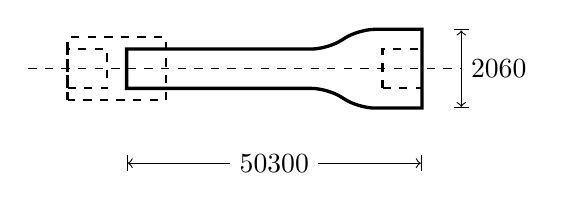
\begin{tikzpicture}[scale=1]
\draw[dashed](-1,0)--(5,0);
\draw[dashed,thick](-.5,-.25)rectangle++(.5,.5);
\draw[dashed,thick](-.5,-.4)rectangle++(1.25,.8)(3.5,-.25)rectangle++(.5,.5);
\draw[very thick](.25,-.25)to(.25,.25)to[rounded corners=2mm](2.8,.25)to[rounded corners=2mm](3.2,.5)to(4,.5)to(4,-.5)to[rounded corners=2mm](3.2,-.5)to[rounded corners=2mm](2.8,-.25)to(.25,-.25)to cycle;
\draw[|<->|](.25,-1.2)--(4,-1.2)node[midway,fill=white]{\numrange{50}{300}};
\draw[|<->|](4.5,-.5)--(4.5,.5)node[midway,fill=white,right]{\numrange{20}{60}};
\end{tikzpicture}